%%%%%%%%%%%%%%%%%%%%%%%%%%%%%%%%%%%%%%%%%
% Stylish Article
% LaTeX Template
% Version 2.1 (1/10/15)
%
% This template has been downloaded from:
% http://www.LaTeXTemplates.com
%
% Original author:
% Mathias Legrand (legrand.mathias@gmail.com) 
% With extensive modifications by:
% Vel (vel@latextemplates.com)
%
% License:
% CC BY-NC-SA 3.0 (http://creativecommons.org/licenses/by-nc-sa/3.0/)
%
%%%%%%%%%%%%%%%%%%%%%%%%%%%%%%%%%%%%%%%%%

%----------------------------------------------------------------------------------------
%	PACKAGES AND OTHER DOCUMENT CONFIGURATIONS
%----------------------------------------------------------------------------------------

\documentclass[fleqn,10pt]{SelfArx} % Document font size and equations flushed left

\usepackage[english]{babel} % Specify a different language here - english by default

\usepackage{lipsum} % Required to insert dummy text. To be removed otherwise

\captionsetup[figure]{justification=justified, singlelinecheck=off} 
\captionsetup[table]{justification=justified, singlelinecheck=off} 
%----------------------------------------------------------------------------------------
%	COLUMNS
%----------------------------------------------------------------------------------------

\setlength{\columnsep}{0.55cm} % Distance between the two columns of text
\setlength{\fboxrule}{0.75pt} % Width of the border around the abstract

%----------------------------------------------------------------------------------------
%	COLORS
%----------------------------------------------------------------------------------------

\definecolor{color1}{RGB}{0,0,90} % Color of the article title and sections
\definecolor{color2}{RGB}{0,20,20} % Color of the boxes behind the abstract and headings

%----------------------------------------------------------------------------------------
%	HYPERLINKS
%----------------------------------------------------------------------------------------

\usepackage{hyperref} % Required for hyperlinks
\hypersetup{hidelinks,colorlinks,breaklinks=true,urlcolor=color2,citecolor=color1,linkcolor=color1,bookmarksopen=false,pdftitle={Title},pdfauthor={Author}}

%----------------------------------------------------------------------------------------
%	ARTICLE INFORMATION
%----------------------------------------------------------------------------------------

% \JournalInfo{Journal, Vol. XXI, No. 1, 1-5, 2013} % Journal information
\JournalInfo{$ $ } % Journal information
\Archive{Pre-print} % Additional notes (e.g. copyright, DOI, review/research article)

\PaperTitle{Numerical Instabilities in Analytical Pipelines Compromise the Reliability of Network Neuroscience} % Article title

\Authors{Gregory Kiar\textsuperscript{1}, Yohan Chatelain\textsuperscript{2}, Pablo de Oliveira Castro\textsuperscript{3},
Eric Petit\textsuperscript{4}, Ariel Rokem\textsuperscript{5}, Gaël Varoquaux\textsuperscript{6},
Bratislav Misic\textsuperscript{1}, Tristan Glatard\textsuperscript{2*$\dagger$},
Alan C. Evans\textsuperscript{1$\dagger$}} % Authors
\affiliation{\textsuperscript{1}\textit{Montréal Neurological Institute, McGill University, Montréal, QC, Canada}} % Author affiliation
\affiliation{\textsuperscript{2}\textit{Department of Computer Science and Software Engineering, Concordia University, Montréal, QC, Canada}} % Author affiliation
\affiliation{\textsuperscript{3}\textit{Department of Computer Science, Université of Versailles, Versailles, France}} % Author affiliation
\affiliation{\textsuperscript{4}\textit{Exascale Computing Lab, Intel, Paris, France}} % Author affiliation
\affiliation{\textsuperscript{5}\textit{Department of Psychology and eScience Institute, University of Washington, Seattle, WA, USA}} % Author affiliation
\affiliation{\textsuperscript{6}\textit{Parietal project-team, INRIA Saclay-ile de France, France}} % Author affiliation
\affiliation{*\textbf{Corresponding author}: tristan.glatard@concordia.ca} % Corresponding author
\affiliation{$\dagger$Authors contributed equally}

\Keywords{Stability --- Reproducibility --- Network Neuroscience --- Neuroimaging} % Keywords - if you don't want any simply remove all the text between the curly brackets
\newcommand{\keywordname}{Keywords} % Defines the keywords heading name

%----------------------------------------------------------------------------------------
%	ABSTRACT
%----------------------------------------------------------------------------------------

\Abstract{The analysis of brain-imaging data requires complex and often non-linear transformations to support findings
on brain function or pathologies. And yet, recent work has shown that variability in the choices that one makes when
analyzing data can lead to quantitatively and qualitatively different results, endangering the trust in
conclusions~\cite{Glen2018-sg,botvinik2020variability,Lewis2017-ll,Glatard2015-vc,salari2020file,Kiar2020-lb}.
Even within a given method or analytical technique, numerical instabilities could compromise findings. We instrumented
a structural-connectome estimation pipeline with Monte Carlo Arithmetic~\cite{Parker1997-qq,Denis2016-wo} and evaluated
the stability of the derived connectomes, their features~\cite{Rubinov2010-fh}, and the impact on a downstream
analysis~\cite{Park2015-uj,Gupta2015-ap}. The stability of results was found to be highly dependent upon which features
of the connectomes were evaluated, and ranged from perfectly stable (i.e. no observed variability across executions) to
highly unstable (i.e. the results contained no trustworthy significant information). The extreme range and variability
in results presented here could severely hamper our understanding of brain function in brain-imaging studies. It also
highlights both the potential impact of basic analytical choices and measure on the reliability of downstream analyses,
and the necessity of stability evaluation as a core component of typical analytical workflows.}

%----------------------------------------------------------------------------------------

\begin{document}

\flushbottom % Makes all text pages the same height
\maketitle % Print the title and abstract box
% \tableofcontents % Print the contents section
\thispagestyle{empty} % Removes page numbering from the first page

%----------------------------------------------------------------------------------------
%	ARTICLE CONTENTS
%----------------------------------------------------------------------------------------

The modelling of brain networks, called connectomics, has shaped our understanding of the structure and function
of the brain across a variety of organisms and scales over the last
decade~\cite{behrens2012human,xia2016connectomic,morgan2013not,van2016comparative,Rubinov2010-fh}.
In humans, these wiring diagrams are obtained \textit{in vivo} through Magnetic Resonance Imaging (MRI), and show
promise towards identifying biomarkers of disease. This can not only improve understanding of so-called
``connectopathies'', such as Alzhiemer's Disease and Schizophrenia, but potentially pave the way for
therapeutics, as well~\cite{fornito2015connectomics,deco2014great,xie2012mapping,filippi2013assessment,van2014brain}.

However, the analysis of brain imaging data relies on complex computational methods and software pipelines. Tools are
trusted to perform everything from pre-processing tasks (i.e. image reconstruction, denoising, and alignment) to
downstream modelling and statistical evaluation. While these tools undoubtedly undergo rigorous evaluation, in the
absence of ground-truth this is often evaluated on bespoke datasets through measures of
reliability~\cite{Bartko1966-tl,Brandmaier2018-tk,bridgeford2020elim,Kiar2018-jt}, proxy outcome statistics, or
agreement with previously existing literature and theory. Importantly, this means that tools are not necessarily of
known or consistent quality, and it is not uncommon that equivalent experiments may lead scientists to the diverging
conclusions, calling into question the stability of these
tools~\cite{botvinik2020variability,Lewis2017-ll,Glatard2015-vc,salari2020file}.

The present study perturbed a series brian imaging studies using structural connectomes and explored the biological
implications of observed instabilities in the results. We accomplished this through the use of Monte Carlo Arithmetic
(MCA)~\cite{Parker1997-qq}, a technique which enables characterization of the sensitivity of a system to small
perturbations. We explored the impact of perturbations through the direct comparision of connectomes, the consistency
of their features, and their eventual application in a neuroscience study. Finally we conclude on the consequences of
the observed instabilities and make recommendations for future work in this area.

\begin{figure*}[hbt]\centering
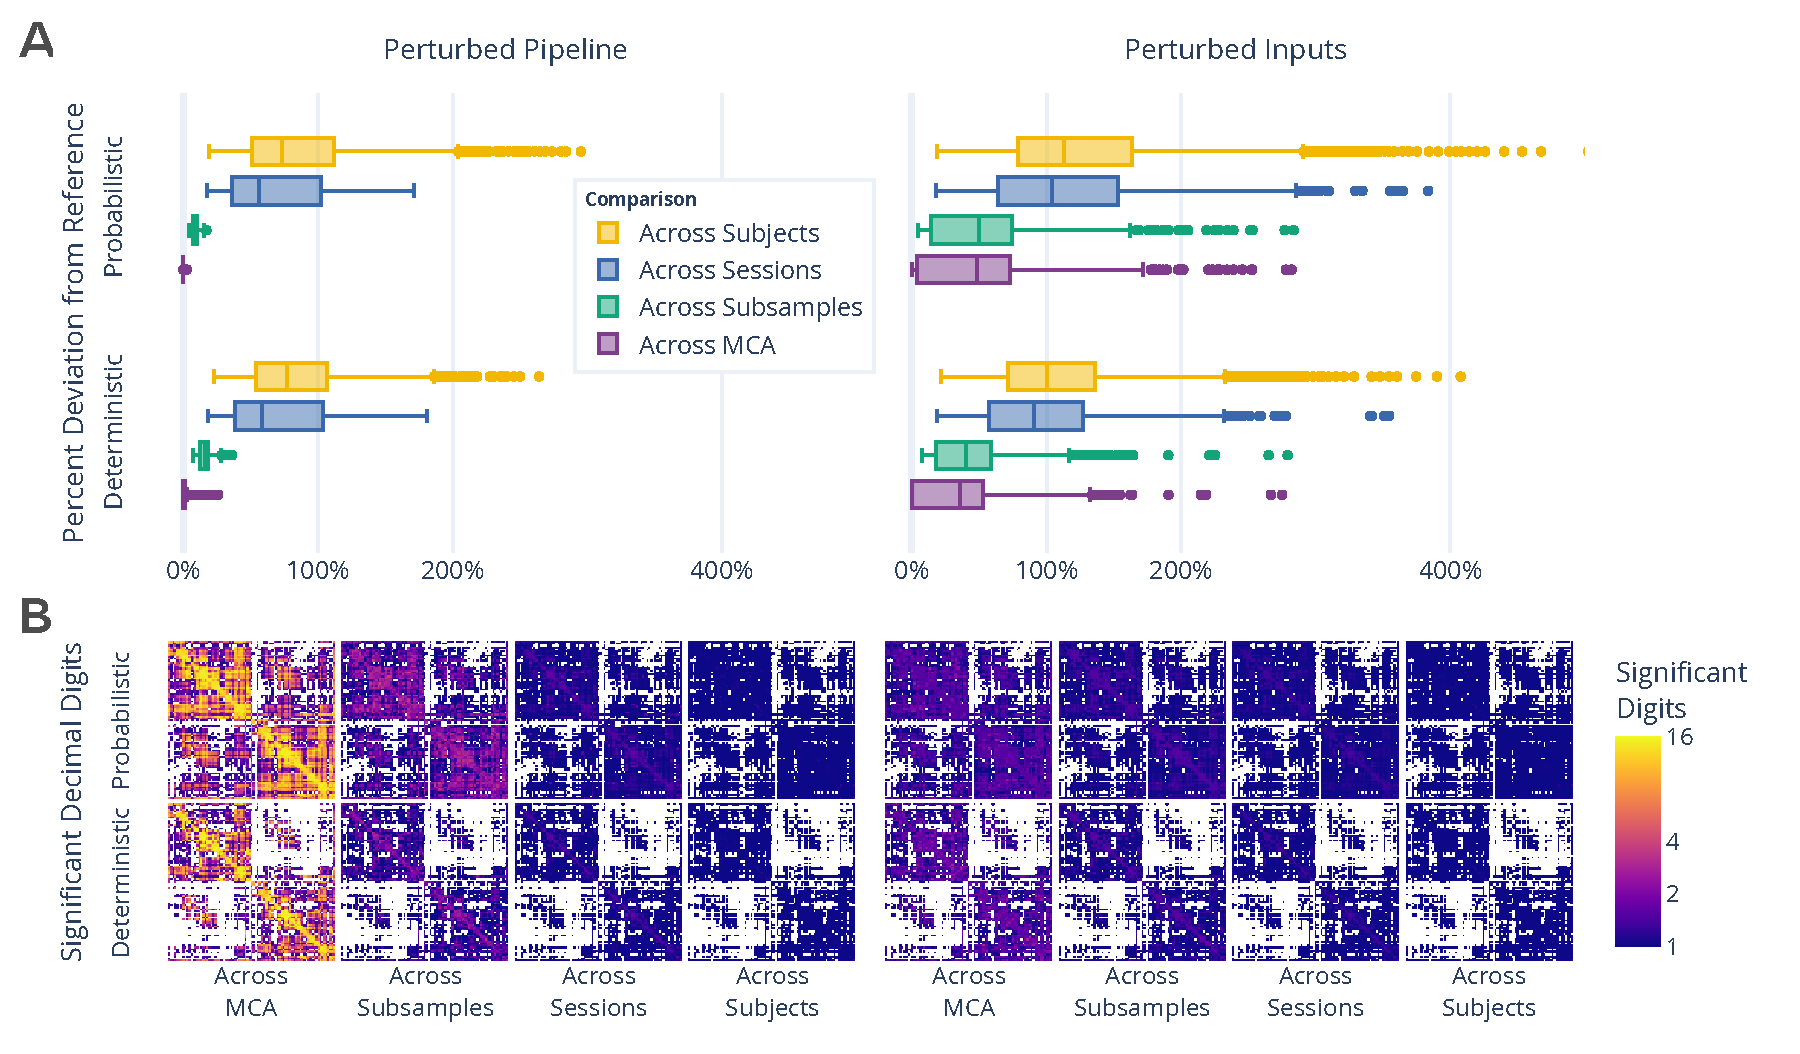
\includegraphics[width=\linewidth]{figures/fig1_absolute_differences.pdf}
\caption{Exploration of perturbation-induced deviations from reference connectomes.
(\textbf{A}) The absolute deviations, in the form of normalized percent deviation from reference, shown as the
across MCA series relative to Across Subsample, Across Session, and Aross Subject variations.
% (\textbf{B}) The correlation between perturbed connectomes and their reference.
(\textbf{B}) The number of significant decimal digits in each set of connectomes as obtained after evaluating the
effect of perturbations. In the case of 16, values can be fully relied upon, whereas in the case of 1 only the first
digit of a value can be trusted. Pipeline- and Input-perturbations are shown on the left and right, respectively.}
\label{fig:absolute}
\end{figure*}


%------------------------------------------------
\subsection*{Graphs Vary Widely With Perturbations}

Figure~\ref{fig:absolute} shows the observed changes in structural connectivity induced by perturbations using two
metrics: percent deviation, and number of significant digits. The deviations observed purely across MCA were displayed
alongside other sources of variability, in order of magnitude, such as: subsampling, variation across sessions, and
variation across subjects. In both the case of Pipeline Perturbation and Input Perturbation settings, the magnitude of
percent deviation between pairs of connectomes (Figure~\ref{fig:absolute}A) across each category is consistent with
this sorting. However, there is a much tighter bound in the distribution of differences in both the cross-MCA and
cross-subsample cases with Pipeline Perturbations, where deviations rarely reach the level of session or individual
variations. Connectomes generated with Input Perturbations show considerably more variability, often reaching
deviations equal to or greater than those observed across individuals or sessions. While both pipelines show similar
distributions in both perturbation settings, the probabilistic pipeline is more stable for cross-MCA and
cross-subsample evaluations in the face of Pipeline Perturbations whereas the deterministic is more stable under Input
Perturbations ($p < 0.0001$ for all; exploratory).

\begin{table*}[ht]\centering
\caption{The impact of instabilities evaluated through the separability of the dataset based on simulation, subsample,
session, and subject (reported as mean~$\pm$~standard deviation Discriminability). While a perfectly separable dataset
would be represented by a score of $1.0$, the chance performance is $1 /$the number of classes. In the case of
Hypothesis 1, the evaluation of similarity across individuals, the chance performance is $0.04$. In the case of
Hypotheses 2 and 3, the evaluation of similarity across sessions or subsamples, respectively, the chance performance is
$0.5$. The alternative hypothesis, indicating significant separation across classes, is accepted for all experiments,
with $p < 0.005$.}
\vspace{5pt}
% \fcolorbox{color1}{white}{%
% \parbox{\textwidth-2\fboxsep-2\fboxrule}{\centering
%   \colorbox{color2!10}{
%     \parbox{\textwidth-4\fboxsep-2\fboxrule}{

\begin{tabular}{llll|ll|ll|ll}
  &  &  &  &  \multicolumn{2}{l|}{\textbf{Reference Execution}} & \multicolumn{2}{l|}{\textbf{Perturbed Pipeline}} &  \multicolumn{2}{l}{\textbf{Perturbed Inputs}} \\
Exp. & Subj. & Sess. & Samp. & Det. &  Prob. &  Det. &    Prob. &     Det. &    Prob. \\
% Exp. & Subj. & Sess. & Dirs. & Sims. &     Discrim. (D) &    Discrim. (P) &     Discrim. (D) &    Discrim. (P) \\
\hline
1.1        &          All &      All &          1 &  $ 0.64 \pm 0.00 $ &  $ 0.65 \pm 0.00 $  &  $ 0.82 \pm 0.00 $ &  $ 0.82 \pm 0.00 $ &  $ 0.77 \pm 0.00 $ &  $ 0.75 \pm 0.00 $ \\
1.2        &          All &        1 &        All &  $ 1.00 \pm 0.00 $ &  $ 1.00 \pm 0.00 $ &  $ 1.00 \pm 0.00 $ &  $ 1.00 \pm 0.00 $ &  $ 0.93 \pm 0.02 $ &  $ 0.90 \pm 0.02 $ \\
1.3        &          All &        1 &          1 &        &  &  $ 1.00 \pm 0.00 $ &  $ 1.00 \pm 0.00 $ &  $ 0.94 \pm 0.02 $ &  $ 0.90 \pm 0.02 $ \\
& & & & & & & & & \vspace{-5pt}\\
2.4        &            1 &      All &        All &  $ 1.00 \pm 0.00 $ &  $ 1.00 \pm 0.00 $  &  $ 1.00 \pm 0.00 $ &  $ 1.00 \pm 0.00 $ &  $ 0.88 \pm 0.12 $ &  $ 0.85 \pm 0.12 $ \\
2.5        &            1 &      All &          1 &        &  &  $ 1.00 \pm 0.00 $ &  $ 1.00 \pm 0.00 $ &  $ 0.89 \pm 0.11 $ &  $ 0.84 \pm 0.12 $ \\
& & & & & & & & & \vspace{-5pt}\\
3.6        &            1 &        1 &        All &         &  &  $ 0.99 \pm 0.03 $ &  $ 1.00 \pm 0.00 $ &  $ 0.71 \pm 0.07 $ &  $ 0.61 \pm 0.05 $ \\
\end{tabular}


%     }
%   }
% }%
% }%

\label{tab:discrim}
\end{table*}

The number of significant digits per edge across connectomes (Figure~\ref{fig:absolute}B) similarly follows the
expected and previously observed trend across groups. While the cross-MCA Pipeline Perturbation evaluations show nearly
perfect precision (approaching $16$ digits) for many edges, this evaluation uniquely shows considerable drop off in
performance with the cross-subsample group (average of $< 4$ digits). The combination of this with results presented in
Figures~\ref{fig:absolute}A suggests that specific edge weights are largely affected by these perturbations while
macro-scale connectivity is largely unchanged. Connectomes perturbed by Input Perturbations show no more than an
average of $3$ significant digits across all groups. In the case of both perturbations, cross-individual significance
does not exceed a single digit per edge, suggesting that groupwise average connectomes should be limited to a single
digit of precision (i.e. only the order of magnitude of the edge can be relied upon).

The fact that each of these direct comparisons show distinct relationships between pipeline, perturbation mode, and
data, illustrates the high dependence of stability evaluation upon specific application context.

\subsection*{Subject-Specific Signal is Amplified While Artifacts Are Reduced}

Beyond direct difference on the connectomes, we evaluated the discriminability between groups, to characterize
quantitatively the impact of perturbations on the separability of the dataset (Table~\ref{tab:discrim}). For
hypothesis 1, which explores the separability of the dataset with respect to participant labels, an ideal dataset would
have a discriminability score of $1.0$. In experiment 1.1, that which mimics a typical test-retest scenario, we observe
that the dataset is separable with a discriminability score of $0.64$ or greater in each of these experiments (all
statistically significant, $p < 0.005$). Both MCA instrumentations significantly increase the discriminability, and
therefore reliability, of the dataset in this experiment ($p < 0.001$ for all). This result impactfully suggests the
utility of both MCA methods for synthesizing more robust and reliable individual estimates of connectivity.

Experiment 1.1 is unsurprisingly the least discriminable test of this hypothesis, as experiments 1.2 and 1.3 rely on
the same session of data, either distinguished by downsampling or perturbations, respectively. Input Perturbations lead
to a decrease in the separability of individuals in these experiments, but the reliability still exceeds the
cross-session case.

Hypothesis 2 considers the separability of connectomes based upon session, rather than subject. In this case,
performance was computed within-individual and aggregated. An ideal test-retest dataset – one where there is no
difference between two observations of an individual – would have a discriminability score of $0.5$ in these
experiments.

The discriminability in both the unperturbed and Perturbed Pipeline settings is $1.0$, meaning that there is a
significant difference between sessions of data. However, while still significant relative to chance, Input
Perturbations lead to considerably lower discriminability, reducing the difference between distinct sessions of data.
This suggests that Input Perturbations reduce session-dependent bias.

Finally, experiment 3.6 evaluates the separability of samples based on subsampling. Similarly to the previous, the
performance is once again computed through analyzing individual sessions of data and aggregating across sessions and
individuals, with an ideal score of $0.5$. While this experiment could not be evaluated using reference executions, the
Pipeline Perturbation performance showed near perfect separation between direction subsamples whereas Input
Perturbations considerably lower this separability towards chance, similar to as was observed in experiments 2.4 and
2.5. This is further evidence which suggests that the Input Perturbations may have an application in obtaining more
robust estimates of individual connectivity, as across each experiment it shows an amplification in meaningful
differences while also showing a reduction in off-target differences.

\subsection*{Distributions of Graph Statistics Are Reliable, Individual Statistics Are Not}

\begin{figure*}[bt!]\centering
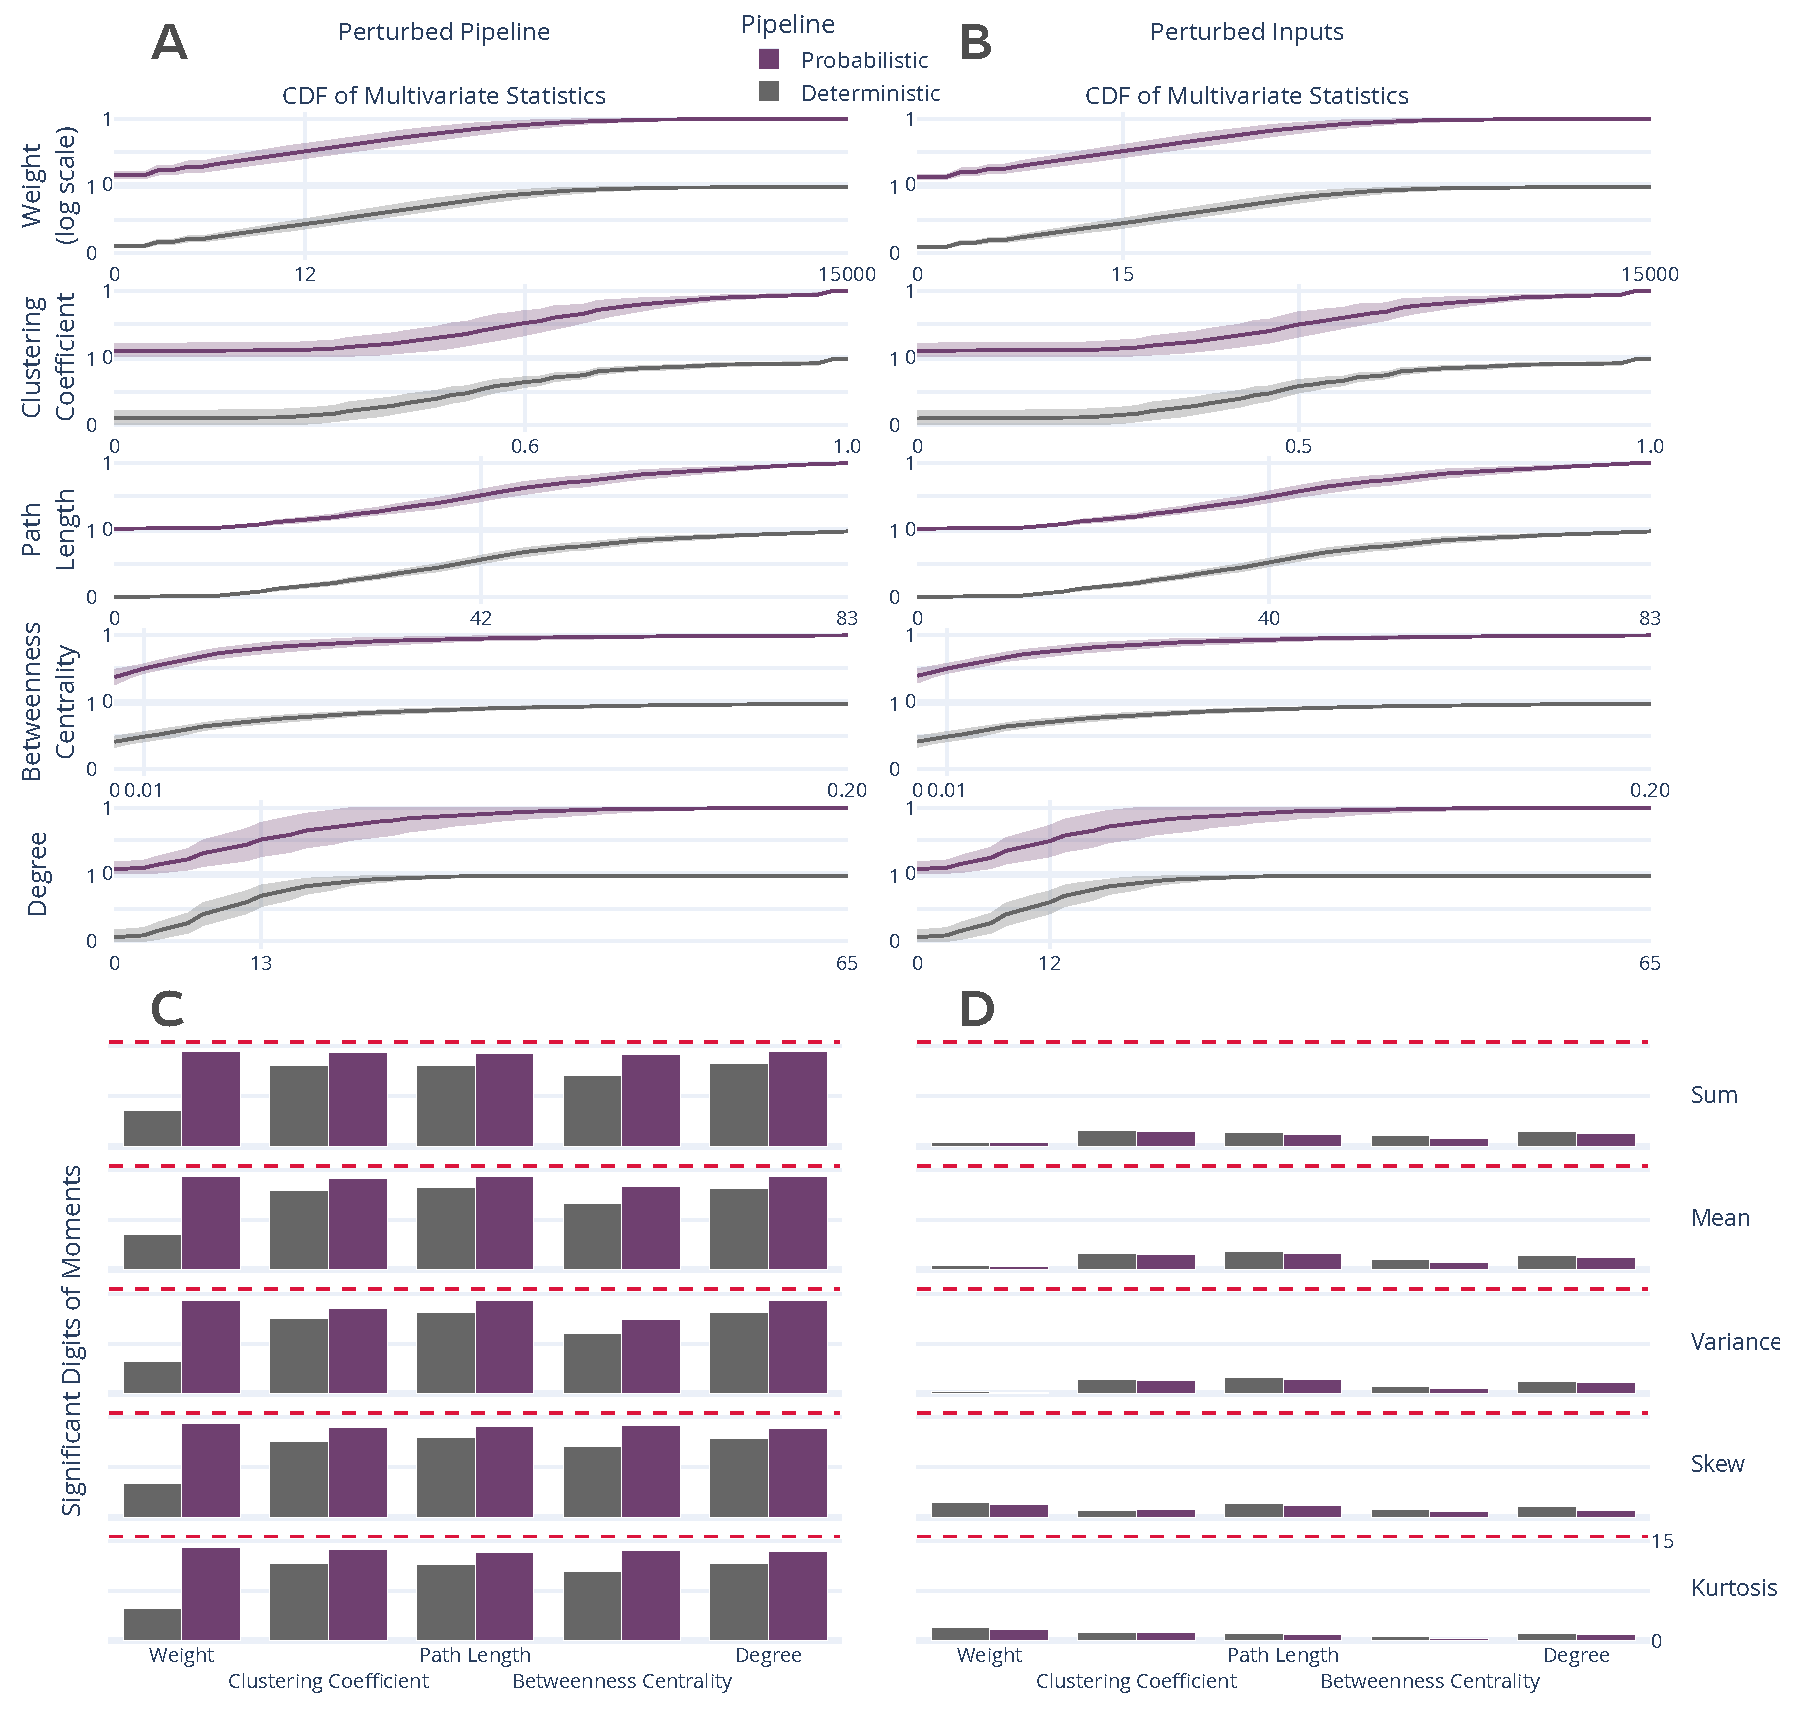
\includegraphics[width=\linewidth]{figures/fig2_multivariate_differences.pdf}
\caption{Distribution and stability assessment of multivariate graph statistics. (\textbf{A}, \textbf{B}) The
cumulative distribution functions of multivariate statistics across all subjects and perturbation settings. There was
no significant difference between the distributions in A and B. (\textbf{C}, \textbf{D}) The number of significant
digits in the first five moments of each statistic across perturbations. The dashed red line refers to the maximum
possible number of significant digits.}
\label{fig:multivar}
\end{figure*}

Connectomes are often summarized by lower-dimensional statistics more suitable for numerous analytical
methods~\cite{Rubinov2010-fh}. Figure~\ref{fig:multivar} explores the stability of these graph-theoretical metrics
computed from the perturbed graphs, including weight, clustering coefficient, path length, betweenness centrality, and
degree. Due to the variable length of the edgewise statistics, cumulative density functions for each statistic were
evaluated over a fixed range and the mean density and associated standard error were computed for each bin
(Figures~\ref{fig:multivar}A and ~\ref{fig:multivar}B), with the distributions' minimum, median, and maximum values
denoted on each x-axis. There was no significant difference in distributions observed for each statistic across the two
perturbation settings. The first 5 moments of these statistics within individuals as observed with Pipeline
Perturbations (Figure~\ref{fig:multivar}C) were stable with more than $10$ significant digits with the exception of
edge weight when using the deterministic pipeline. In the case of all statistics, the probabilistic pipeline was more
stable than the deterministic pipeline ($p < 0.0001$; exploratory). In stark contrast, these moments were highly
unstable in the face of Input Perturbations (Figure~\ref{fig:multivar}D), in which no measure had more than $5$
significant digits of information, and several moment and statistic pairs had less than a single significant digit,
such as the variance in edge weight or the kurtosis of betweenness centrality. In general, there was not a strong
relationship between the order of the moment and its stability. A similar analysis was performed for univariate
statistics in \sref{supsec:univar}.

The large discrepancy between the stability of individual estimates in these settings versus the similarity of
aggregated CDFs suggests that while individual estimates are unstable, the comparison between aggregates or groups may
be considered much more reliable.

\subsection*{The Strength of Brain-Behaviour Relationships is Eroded}

\begin{figure*}[ht]\centering
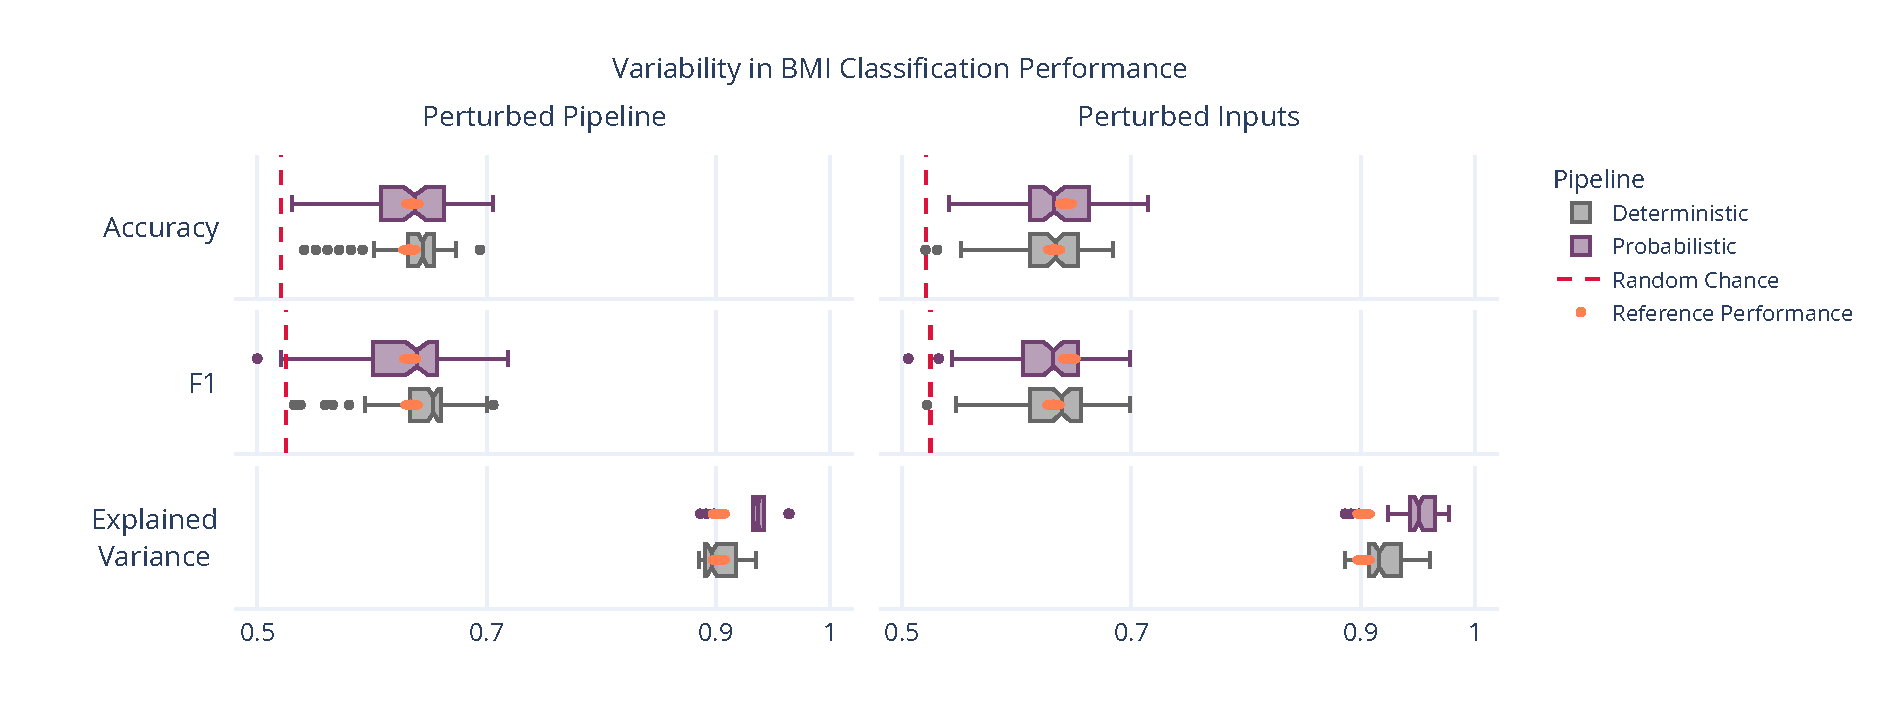
\includegraphics[width=\linewidth]{figures/fig3_bmi_classification.pdf}
\caption{Observed variability in BMI classification. Training and Test sets were sampled from the MCA-generated dataset
such that a single observation of each individual was present in each sampling. This sampling was performed 20 times,
and each dataset was used to train a classifier with each of 2, 5, 10, and N-fold cross validation, and the shown
metrics are the average across each of these training paradigms. The dashed red lines indicate random-chance
performance, and the orange dots show the performance using the reference executions.}
\label{fig:bmi}
\end{figure*}

While the variability of explicit features of connectomes was summarized above, these networks are commonly-used as
inputs to machine learning models. Here, connectomes were projected into a low dimensional space using PCA and then
input a logistic regression classifier (Figure~\ref{fig:bmi}). The number of principal components was selected as the
minimum number of components required to capture 90\% of the variance in the reference set; this resulted in $20$
components. Using the reference performance, i.e. that using only unperturbed graphs (Figure~\ref{fig:bmi}; orange
overlay), the classification accuracies were $0.635$ and $0.628$, and the F1 scores were $0.636$ and $0.630$ for data
derived using the deterministic and probabilistic pipelines, respectively, with the average explained variance at 90\%
in both cases. The random chance performance for these evaluations measures were $0.521$ and $0.519$, respectively
(Figure~\ref{fig:bmi}; dashed red line).

When performing this analysis using sampled instances of the perturbed dataset across both pipelines and perturbation
methods, the portion of explained variance in the sample with $20$ components ranged from $0.886$ -– $0.978$. The
classification accuracy ranged from $0.520$ – $0.716$ and the F1 score ranged from $0.510$ -– $0.725$. These results
range from at or below random chance performance, to considerable accuracy that outperforms that obtained using the
reference dataset.

\begin{equation}
\cos^3 \theta =\frac{1}{4}\cos\theta+\frac{3}{4}\cos 3\theta
\label{eq:refname2}
\end{equation}

\lipsum[5] % Dummy text

\begin{enumerate}[noitemsep] % [noitemsep] removes whitespace between the items for a compact look
\item First item in a list
\item Second item in a list
\item Third item in a list
\end{enumerate}

\lipsum[14] % Dummy text

\begin{itemize}[noitemsep] % [noitemsep] removes whitespace between the items for a compact look
\item First item in a list
\item Second item in a list
\item Third item in a list
\end{itemize}

\subsection{Discussion}
{\color{orange}Notes\\\\
You could mention that instabilities affect not only the topology, but the geometry of reconstructed networks.

It means that we are, as a field, overconfident in numerical stability, and that in a typical setting this would lead
to wrong conclusions. Or am I over-stating it? Because if that's the case, it needs to be unequivocally stated here.
And in the abstract. And maybe also in the title of the article. this amount of numerical noise is to be expected in
typical settings, not only in MCA. Is that correct? And that has implications for inferences in the typical setting.
}

%----------------------------------------------------------------------------------------
%	REFERENCE LIST
%----------------------------------------------------------------------------------------
\phantomsection
\bibliographystyle{IEEEtran}
\bibliography{impact-of-instability}

\section*{Methods}
\lipsum[10]

%------------------------------------------------
\phantomsection
\subsection*{Author Contributions}
GK was responsible for the experimental design, data processing, analysis, interpretation, and the majority of writing.
All authors contributed to the revision of the manuscript. YC, POC, and EP were responsible for MCA tool development
and software testing. AR, GV, and BM contributed to experimental design and interpretation. TG contributed to
experimental design, analysis, and interpretation. TG and ACE were responsible for supervising and supporting all
contributions made by GK. The authors declare no competing interests for this work.

\subsection*{Acknowledgments} 
This research was financially supported by the Natural Sciences and Engineering Research Council of Canada (NSERC)
(award no. CGSD3-519497-2018). This work was also supported in part by funding provided by Brain Canada, in partnership
with Health Canada, for the Canadian Open Neuroscience Platform initiative.

\subsection*{Additional Information}
Supplementary Information is available for this paper. Correspondence and requests for materials should be addressed to
Tristan Glatard at \url{tristan.glatard@concordia.ca}.

%----------------------------------------------------------------------------------------
\beginsupplement

\clearpage
\section{Graph Correlation}
\label{supsec:correlation}
The correlations between observed graphs (Figure 1B) across each grouping follow the same trend to percent deviation.
However, notably different from percent deviation, there is no significant difference in the correlations between
Pipeline or Input instrumentations. By this measure, the probabilistic pipeline is more stable in all cross-MCA and
cross-directions except for the combination of Input Perturbation and cross-MCA (p < 0.0001 for all; exploratory).

\begin{figure}[ht]\centering
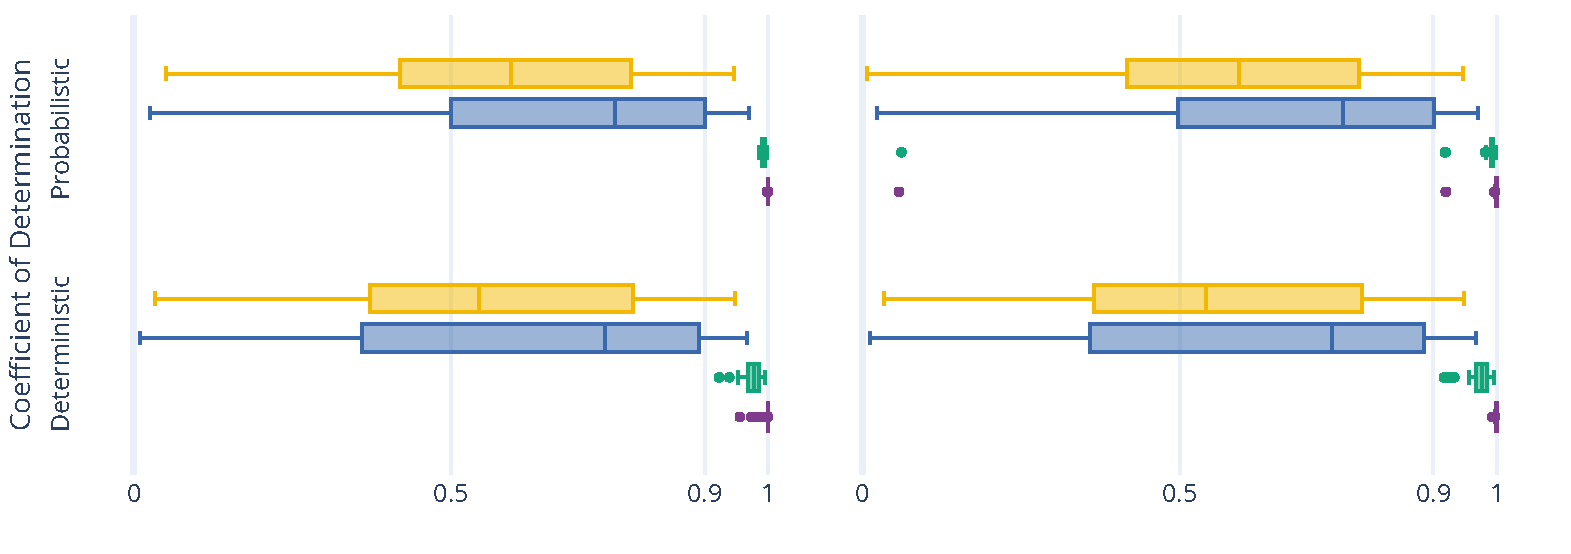
\includegraphics[width=\linewidth]{figures/figS1_correlation_differences.pdf}
\caption{The correlation between perturbed connectomes and their reference.}
\label{fig:correlation}
\end{figure}

\clearpage
\section{Univariate Graph Statistics}
\label{supsec:univar}

Figure 2 explores the stability of these graph-theoretical metrics computed from the perturbed graphs, including
modularity, global efficiency, assortativity, average path length, and edge count. When aggregated across individuals
and perturbations, the distributions of these statistics (Figures 2A and 2B) show no significant differences between
perturbation methods for either deterministic or probabilistic pipelines. However, when quantifying the stability of
these measures across connectomes derived from a single session of data, the two perturbation methods show considerable
differences. The number of significant digits in univariate statistics for Pipeline Perturbation instrumented
connectome generation exceeded 11 digits for all measures except modularity, which contained more than 4 significant
digits of information (Figure 2C). When detecting outliers from the distributions of observed statistics for a given
session, the false positive rate (using a threshold of p = 0.05) was approximately 2\% for all statistics with the
exception of modularity which again was less stable with an approximately 10\% false positive rate. The probabilistic
pipeline is significantly more stable than the deterministic pipeline (p < 0.0001; exploratory) for all features
except modularity. When similarly evaluating these features from connectomes generated in the Input Perturbation
setting, no statistic was stable with more than 3 significant digits or a false positive rate lower than nearly 6\%
(Figure 2D). The deterministic pipeline was more stable than the probabilistic pipeline in this setting (p < 0.0001;
exploratory).

Two notable differences between the two perturbation methods are, first, the uniformity in the stability of the
statistics, and second, the dramatic decline in stability of individual statistics in the Input Perturbation setting
despite the consistency in the overall distribution of values. It is unclear at present if the discrepancy between the
stability of modularity in the Pipeline Perturbation context versus the other statistics suggests the implementation of
this measure is the source of instability or if it is implicit to the measure itself. The dramatic decline in the
stability of features derived from Input Perturbed graphs despite no difference in their overall distribution both
shows that while individual estimates may be unstable the comparison between aggregates or groups may be considered
much more reliable.

\begin{figure}[ht]\centering
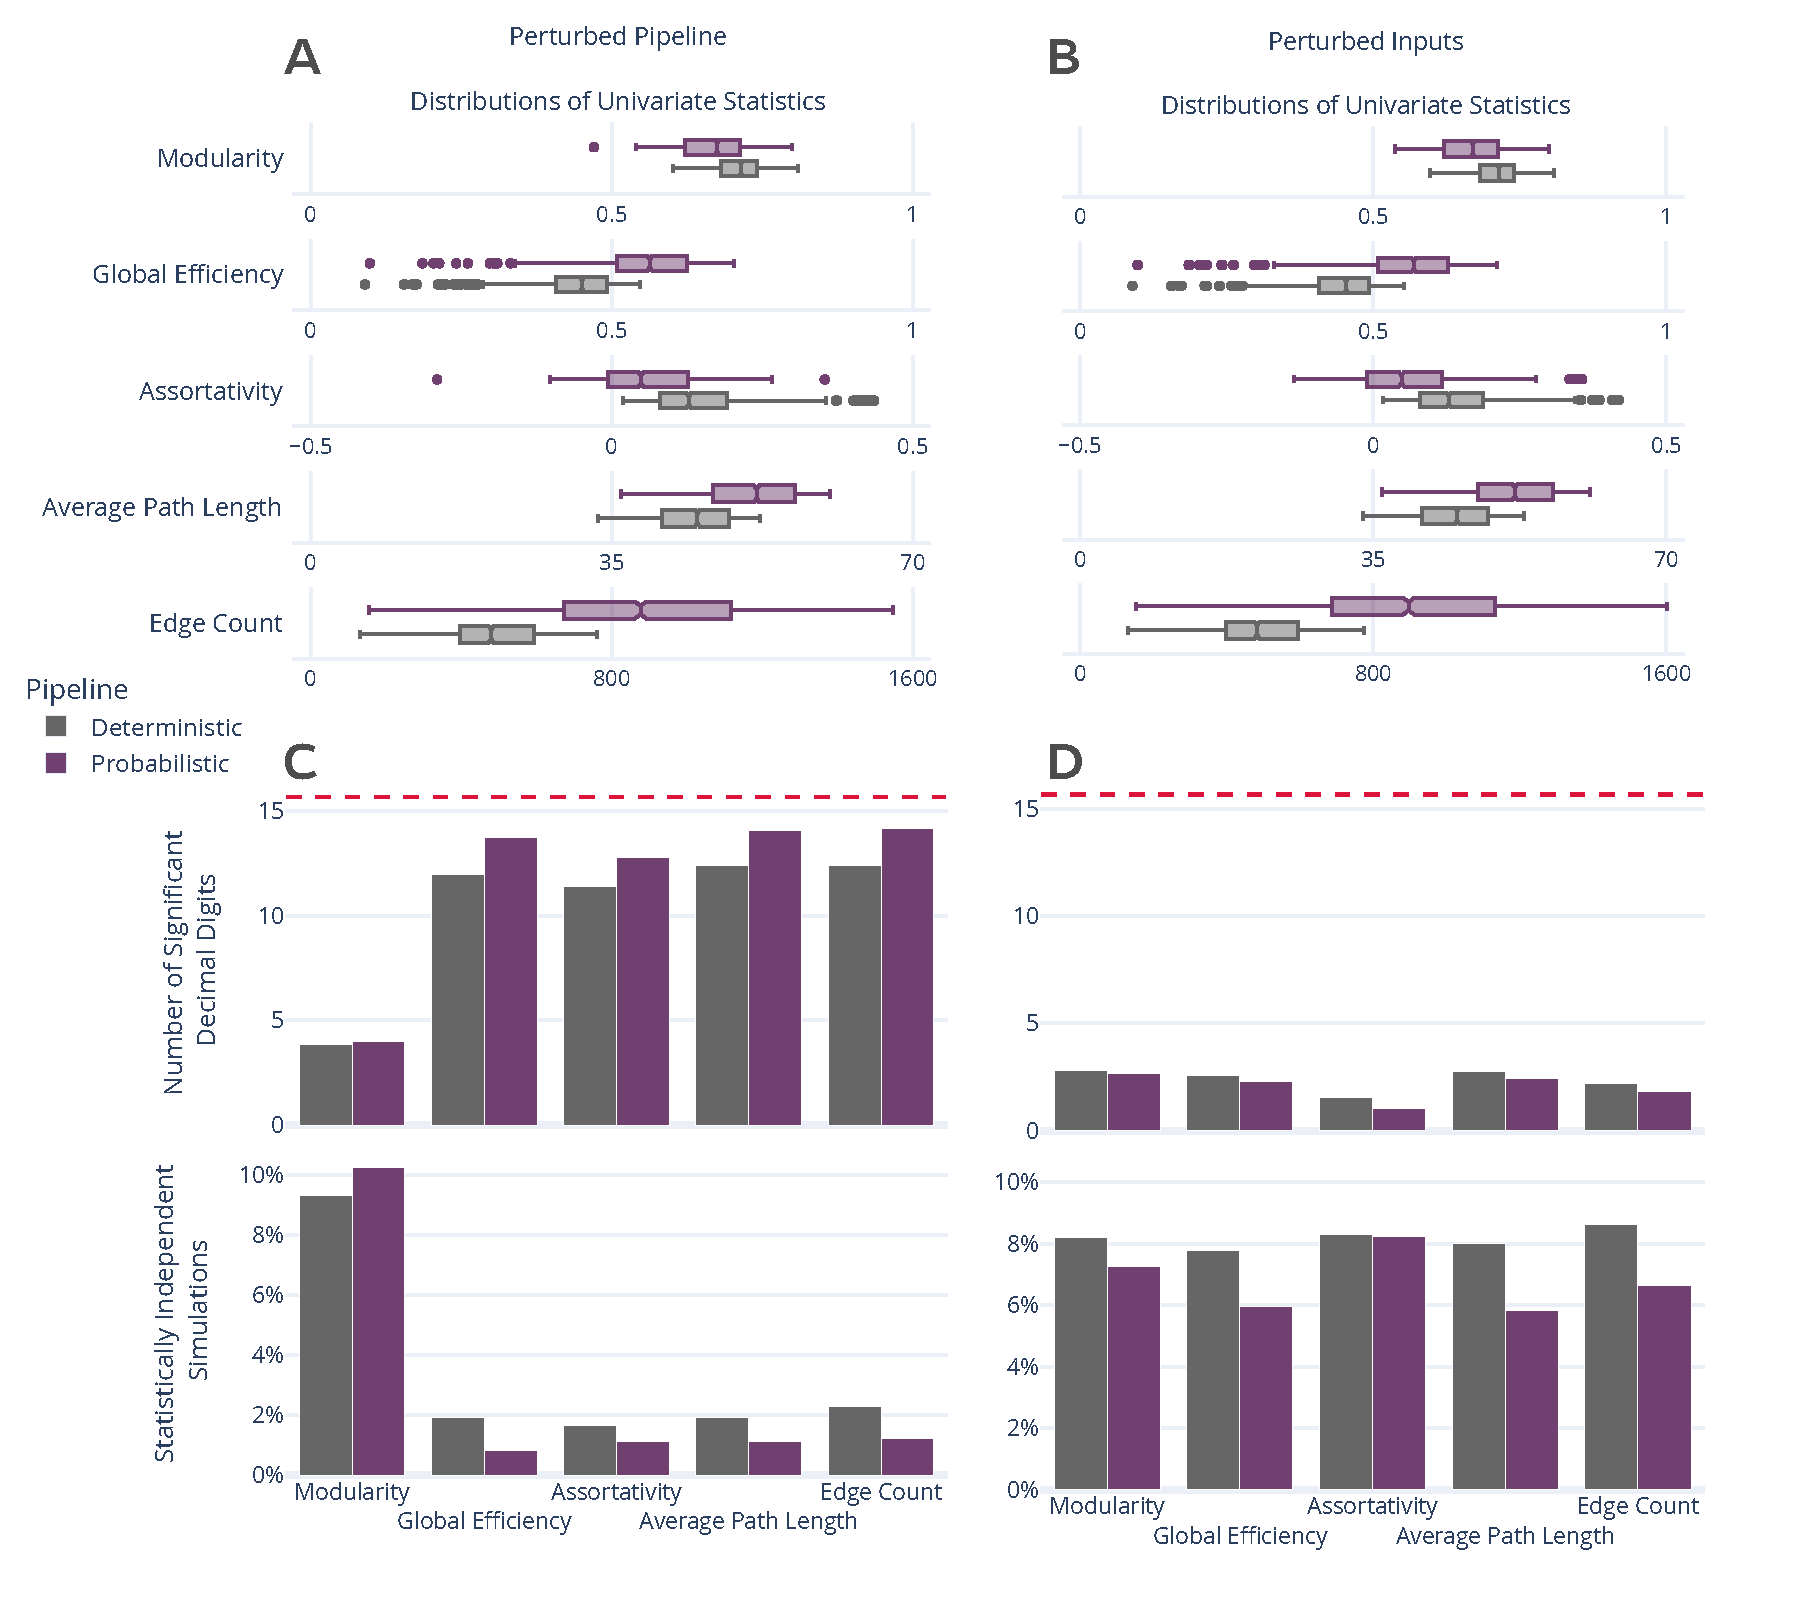
\includegraphics[width=\linewidth]{figures/figS2_univariate_differences.pdf}
\caption{Distribution and stability assessment of univariate graph statistics. (\textbf{A}, \textbf{B}) The
distributions of each computed univariate statistic across all subjects and perturbations for Pipeline and Input
settings, respectively. There was no significant difference between the distributions in A and B. (\textbf{C},
\textbf{D}; top) The number of significant decimal digits in each statistic across perturbations, averaged across
individuals. The dashed red line refers to the maximum possible number of significant digits.
(\textbf{C}, \textbf{D}; bottom) The percentage of connectomes which were deemed significantly different
($p < 0.05$) from the others obtained for an individual.}
\label{sfig:univariate}
\end{figure}


\end{document}
